%!TEX root = ../thesis.tex

\chapter{Resultados}

\ifpdf
    \graphicspath{{resultados/Figs/Raster/}{resultados/Figs/PDF/}{resultados/Figs/}}
\else
    \graphicspath{{resultados/Figs/Vector/}{resultados/Figs/}}
\fi

El proyecto logró producir una herramienta que permite la creación de juegos en lenguaje Haskell. Para poder comprobar su funcionalidad y desempeño se hace uso de programas de ejemplo creados usando la herramienta.

\section{Ejemplo motor gráfico}

Para la prueba del motor gráfico se creó un programa que dibuja en pantalla el armadillo de Stanford en color amarillo. Este programa no tiene ninguna clase de interacción. Se puede ver el programa en la sección de código Ejemplo1~\ref{Ejemplo1}, el código requerido para este programa es sencillo y corto gracias al motor.

\begin{figure}[htbp!]
\centering
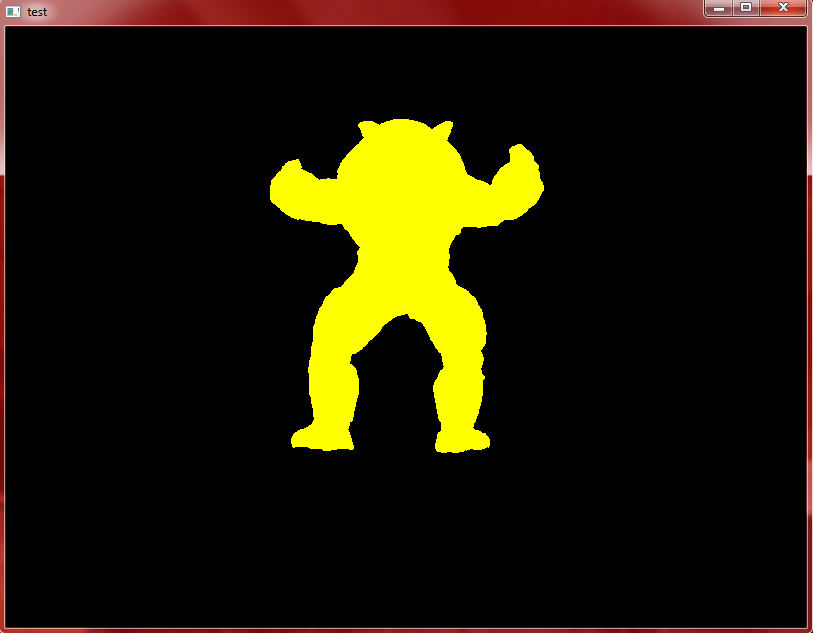
\includegraphics[width=1.0\textwidth]{sceenshot1}
\caption[Ejemplo 1]{El armadillo de Stanford dibujado en color amarillo.}
\end{figure}

\section{Ejemplo motor de juego}

El motor de juego se prueba mediante un programa que crea un número de esferas que se mueven en alguna dirección e invierten la dirección en la que se mueven cuando colisionan con otra esfera o llegan al límite de un área predefinida. Este ejemplo se puede encontrar en la sección de código Ejemplo2~\ref{Ejemplo2}.

Para este ejemplo se observa los FPS (frames per second) del programa con diferente cantidad de esferas y permitiendo al RTE de haskell correr con una cantidad diferente de hilos máximos. Esta prueba permitirá observar el rendimiento y el uso de paralelismo del motor de juego en diversas situaciones.

\begin{table}
\begin{tabular}{ | l | c | c | c | c | }
 \hline
 FPS & 1 hilo &2 hilos&3 hilos&4 hilos\\
 \hline
 5 esferas & 1550	& 1650	& 1820	& 1780 \\ \hline
 10 esferas & 1350	& 1480	& 1550	& 1520 \\ \hline
 50 esferas & 430	& 520	& 650	& 620 \\ \hline
 100 esferas & 212	& 270	& 350	& 340 \\ \hline
 200 esferas & 100	& 150	& 160	& 160 \\ \hline
 400 esferas & 42	& 68	& 72	& 72 \\ \hline
 600 esferas & 27	& 40	& 44	& 44 \\
 \hline
\end{tabular}
\caption{FPS en corridas de Ejemplo 2.}
\label{table:Ejemplo2}
\end{table}

En la tabla~\ref{table:Ejemplo2} se observa, como era de esperarse, una disminución de los FPS a medida que se aumenta el número de entidades en la escena. Pero gracias al uso de paralelismo del motor, el uso de hilos adicionales permite aumentar el número de FPS por cantidad de entidades. Los datos muestran que el programa corre a mayor velocidad cuando se utilizan tres hilos de cómputo, en especial en los casos con pocas entidades.

En los casos con pocas entidades, la caída en FPS puede atribuirse al costo incurrido en crear y destruir hilos siendo mayor a la ganancia de procesar las entidades en hilos separados. Sin embargo, cuando se aumenta el número de entidades, los FPS con tres y cuatro hilos se hacen iguales en lugar de aumentar, en la sección ~\ref{sec:Escenas} se establece que el hilo lógico usa la librería Control.Parallel.Strategies para realizar la actualización de las entidades en paralelo, el motor de juego posee, en la implementación actual, tres hilos que siempre se encuentran activos, cualquier otro hilo es creado en base a demanda. Ello significa que al usar tres hilos el RTE de Haskell corra la actualización de las entidades en el hilo asignado al hilo lógico, pero al haber cuatro, el RTE puede estar incurriendo en un problema en el que administrar que tareas asignar a este hilo disponible sea más caro que la tarea siendo asignada al hilo. La otra posible causa de no aprovecharse el cuarto hilo yace en que la estrategia usada de la librería Control.Parallel.Strategies no esté llevando los objetos a forma normal, en haskell eso significa que un cómputo este totalmente computado y no sea una promesa, que podría ser resuelto cambiando de estrategia e implementando la clase NFData para el tipo de dato ObjOutput.

Este ejemplo muestra que el uso de hilos en el motor provee de mayor rendimiento a los juegos creados sin aumentar la complejidad del motor. Es recomendable para cualquier funcionalidad adicional que se agregue al motor, el implementarse un hilo separado que solo dependa del estado del juego.

\begin{figure}[htbp!]
\centering
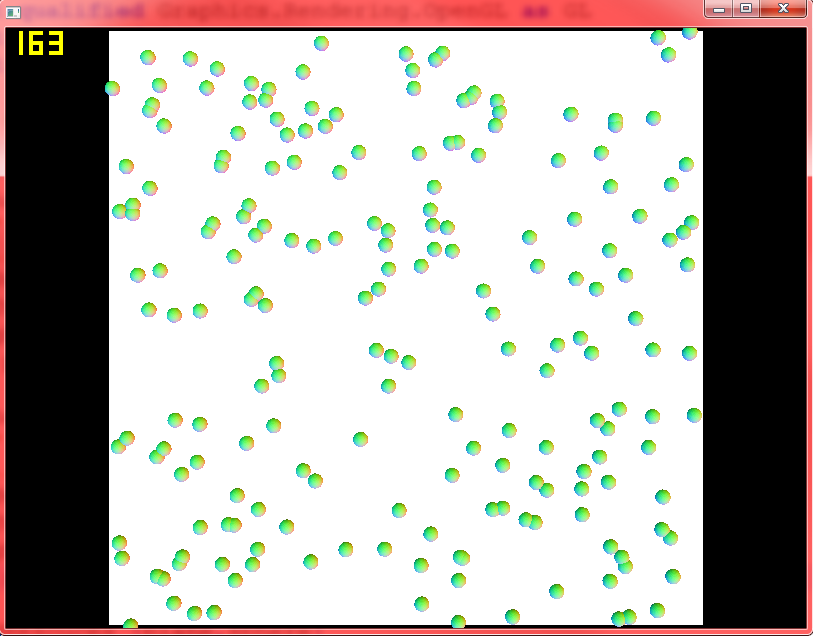
\includegraphics[width=1.0\textwidth]{sceenshot2}
\caption[Ejemplo 2]{200 esferas.}
\end{figure}

\section{Sobre GLUT y OpenGL}

El uso de monads para expresar las operaciones relativas a GLUT resulta como una manera más cómoda y segura para interactuar con la librería según la experiencia adquirida en el uso del monad. Esta experiencia es consistente con un caso similar en el cual Facebook uso monads y Aplicative (clase de haskell) para expresar cómputos paralelos en sus reglas de filtrado de spam, que gracias a la notación de monad de haskell hace el código más limpio y seguro \cite{marlow2014there} \cite{Facebook:Fighting} \cite{Facebook:sourcing}.

De la misma forma en la que se logró crear un monad para GLUT,  debe ser posible crear uno similar para OpenGL, que al igual que GLUT comparte muchas similitudes en funcionamiento. Actualmente, la implementación actual no monádica de OpenGL fuerza a que todas las llamadas a funciones de OpenGL deban realizarse en monad IO, lo cual es considerado peligroso ya que cualquier tipo de código puede ser ejecutado en dicho entorno, y al OpenGL tener que correr en IO, es necesario tener que incluir al monad GLUT en la clase MonadIO (que permite a cualquier monad correr IO) para poder correr código OpenGL en el ciclo de ejecución de GLUT, arruinando en cierta medida la idea de seguridad que se esperaba para el monad GLUT.

De poder implementarse un monad para OpenGL, se podría eliminar toda posibilidad de hacer IO en las secciones de código que pertenezcan a GLUT y a OpenGL, lo cual, si bien puede parecer restrictivo, ayudaría a que el monad garantice consistencia en los contextos de ambas librerías \cite{hughes2000generalising}.

La razón principal por la cual un monad no fue implementado para OpenGL es, primero, la librería OpenGL es proporcionalmente más grande y compleja que GLUT. Segundo, en OpenGL se pueden crear objetos únicos de esta librería (ejemplo: VOBs) y su administración y almacenamiento es un tema de discusión, ya que de ser dejado al usuario se rompe la idea de que un monad OpenGL maneje todo el contexto de OpenGL, y dejado como responsabilidad de un posible monad, es difícil dar con una interfaz que resulte cómoda y llamativa para el usuario.
